\subsection{Properties of complete binary tree}
\index{Properties of complete binary tree}
A binary tree is a hierarchical tree type data structure where every node has at most 2 children and in a proper\textbackslash complete binary tree every internal nodes has exactly 2 child nodes. \\
Properties of binary tree:
\begin{itemize}
	\item Special type of binary tree which every level, except possibly the last, is completely filled and all nodes are as far left as possible.
	\item At each level, there are exactly $2^l$ child nodes at level \enquote*{l} where root is assumed as level 1.
	\item Height of that tree is $\log(n+1)$ where n is the number of nodes in the tree.
\end{itemize}

\subsection{Constructed binary tree}
\index{A binary tree constructed from given traversals}
Preorder: \{11, 5, 3, 8, 16, 14, 18, 17, 20\}\\
Inorder: \{3, 5, 8, 11, 14, 16, 17, 18 , 20\}
\begin{figure}[h!]
	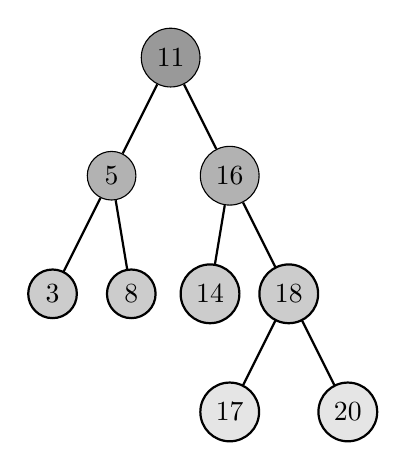
\begin{tikzpicture}[edge from parent/.style={draw, thick}]
		\node[fill=gray!80, circle, draw](11) {11} [grow=down]
	 		child {node[fill=gray!60, circle, draw](5) {5}
	 			child {node[fill=gray!40, circle, draw](3) {3}}
	 			child {node[fill=gray!40, circle, draw, right of=3](8) {8}}}
	 		child {node[fill=gray!60, circle, draw](16) {16}
	 		    child {node[fill=gray!40, circle, draw, right of=8](14) {14}}
	 			child {node[fill=gray!40, circle, draw](18) {18}
	 				child {node[fill=gray!20, circle, draw](17) {17}}
	 				child {node[fill=gray!20, circle, draw](20) {20}}}};
	\end{tikzpicture}
\centering
\caption{Binary tree with given traversals}
\end{figure}